\begin{figure}[h]
\resizebox{\textwidth}{!}{%
%\centering
\begin{subfigure}{0.6\textwidth}
\centering
\begin{tikzpicture}
%\Text[x=0,y=3]{\textbf{HON}}
\Vertex[color=red,x=-2,y=-2,label={$m_{1}$},size=0.8,fontscale=1]{r1}
\Vertex[color=red,x=0,y=-2,label={$m_{2}$},size=0.8,fontscale=1]{r2}
\Vertex[color=red,x=2,y=-2,label={$m_{3}$},size=0.8,fontscale=1]{r3}
\Vertex[color=blue,x=-3,y=1,fontcolor=white,label={$r_{1}$},size=0.8,fontscale=1]{c1}
\Vertex[color=blue,x=-1,y=1,fontcolor=white,label={$r_{2}$},size=0.8,fontscale=1]{c2}
\Vertex[color=blue,x=1,y=1,fontcolor=white,label={$r_{3}$},size=0.8,fontscale=1]{c3}
\Vertex[color=blue,x=3,y=1,fontcolor=white,label={$r_{4}$},size=0.8,fontscale=1]{c4}
\Edge[label=$+$,distance=0.7,lw=1pt](r1)(c1)
\Edge[label=$-$,distance=0.7,lw=1pt](r1)(c2)
\Edge[label=$-$,distance=0.7,lw=1pt](r2)(c1)
\Edge[label=$-$,distance=0.7,lw=1pt](r2)(c2)
\Edge[label=$-$,distance=0.7,lw=1pt](r3)(c2)
\Edge[label=$+$,distance=0.7,lw=1pt](r3)(c3)
\Edge[label=$+$,distance=0.7,lw=1pt](r1)(c4)
\Edge[label=$+$,distance=0.7,lw=1pt](r3)(c4)
%\Edge[Direct,lw=2pt,bend=15](1)(1C)
\end{tikzpicture}
\caption{Signed bipartite network}
\label{fig:ex_a}
\end{subfigure}
\newline
\begin{subfigure}{0.3\textwidth}
\centering
\begin{tikzpicture}
%\Text[x=0,y=3]{\textbf{HON}}
\Vertex[color=red,x=-2.5,y=-0.5,label={$m_{1}$},size=0.8,fontscale=1]{r1}
\Vertex[color=red,x=-0.5,y=-0.5,label={$m_{2}$},size=0.8,fontscale=1]{r2}
\Vertex[color=red,x=-1.5,y=1.5,label={$m_{3}$},size=0.8,fontscale=1]{r3}
\Edge[label=${+,-}$,distance=0.5,lw=1pt](r1)(r2)
\Edge[label=${+,+}$,distance=0.5,lw=1pt](r1)(r3)
\Edge[label=$-$,distance=0.5,lw=1pt](r2)(r3)
\end{tikzpicture}
%\vspace{20pt}
\caption{}Projection onto the methylated DNAs
\label{fig:ex_b}
\end{subfigure}
\begin{subfigure}{0.3\textwidth}
\centering
\begin{tikzpicture}
\Vertex[color=blue,x=0.5,y=-0.5,fontcolor=white,label={$r_{1}$},size=0.8,fontscale=1]{c1}
\Vertex[color=blue,x=2.5,y=-0.5,fontcolor=white,label={$r_{2}$},size=0.8,fontscale=1]{c2}
\Vertex[color=blue,x=0.5,y=1.5,fontcolor=white,label={$r_{3}$},size=0.8,fontscale=1]{c3}
\Vertex[color=blue,x=2.5,y=1.5,fontcolor=white,label={$r_{4}$},size=0.8,fontscale=1]{c4}
\Edge[label=${+,-}$,distance=0.5,lw=1pt](c1)(c2)
\Edge[label=$+$,distance=0.7,lw=1pt](c1)(c4)
\Edge[label=$-$,distance=0.3,lw=1pt](c2)(c3)
\Edge[label=${-,-}$,distance=0.5,lw=1pt](c2)(c4)
\Edge[label=$+$,distance=0.5,lw=1pt](c3)(c4)
\end{tikzpicture}
%\vspace{20pt}
\caption{Projection onto the RNAs}
\label{fig:ex_c}
\end{subfigure}
}
\caption{Exemple of signed bipartite network and its projections.}
\label{fig:toynet}
\end{figure}